% in PDF konfertieren mit (mehrfachdurchläufe notwendig) :! pdflatex %

\documentclass[a4paper, 11pt]{article}

\usepackage[utf8]{inputenc} % für Umlaut-Encoding
\usepackage{ngerman} % für deutsche Titel, Silbentrennung, etc. (benötigt das 
                     % Paket texlive-lang-german)
\usepackage{graphicx} % für Bildeinbindung
\usepackage[round]{natbib} % für das Literaturverzeichnis
\usepackage{acronym} % für das Abkürzungsverzeichnis (benötigt das Paket
                     % texlive-latex-extra)
\usepackage{multirow} % für Tabellen mit spaltenübergreifenden Werten
\usepackage{nonfloat} % für Tabellen/Bild-Positionierung
\usepackage[autostyle=true,german=quotes]{csquotes} % Anführungszeichen global
                                                    % definieren
\usepackage[hidelinks]{hyperref} % für URLs

\title{Grobspezifikation 0.7 \textit{Google Muddle}}
\author{Manuel Mästinger\\\small Modularbeit 4.2 Software Engineering\\\small
ZHAW, School of Engineering, MAS Informatik 8}

\begin{document}

\maketitle
\newpage

\section*{Änderungsverlauf}

Tabelle \ref{tbl:aenderungen} zeigt Änderungen, die im Verlauf der Bearbeitung
an diesem Dokument vorgenommen wurden.
\\[\intextsep]
\begin{minipage}{\linewidth}
	\centering
	\begin{tabular}{rlll}
		\hline
		Version & Beschreibung                                  & Datum       \\
		\hline
		0.1     & Dokument strukturiert                         & 10.05.2015  \\
		0.2     & Einleitung geschrieben                        & 11.05.2015  \\
		0.3     & Systemabgrenzung geschrieben                  & 11.05.2015  \\
		0.4     & Anwendungsfälle modelliert                    & 17.05.2015  \\
		0.5     & Ablaufbeschreibungen erstellt                 & 14.06.2015  \\
		0.6     & Klassendiagramm erstellt und beschrieben      & 15.06.2015  \\
		0.7     & Dokument überarbeitet                         & 17.06.2015  \\
		\hline
	\end{tabular}
	\tabcaption{Änderungen am Dokument}
	\label{tbl:aenderungen}
\end{minipage}


\newpage

\tableofcontents
\newpage

\section{Einleitung}
\label{sec:einleitung}

\subsection{Zum Dokument}

Dieses Dokument soll als möglichst präzise und vollständige Vorlage für die
Feinspezifikation der Applikation \textit{Google Muddle} dienen.

In Kapitel \ref{sec:systemabgrenzung} wird das System \textit{Google Muddle}
gegen aussen abgegrenzt. Basierend auf den funktionalen Anforderungen aus dem
Pflichtenheft werden dann in diesem Dokument Anwendungsfälle (Kapitel
\ref{sec:anwendungsfaelle}) definiert. Anschliessend werden alle Schnittstellen
des Systems (Kapitel \ref{sec:systemschnittstellen}) spezifiziert. In Kapitel 
\ref{sec:ablaufbeschreibung} wird dann der Ablauf jedes Anwendungsfalles in
einem Diagramm dargestellt und beschrieben. Und in Kapitel
\ref{sec:klassendiagramm} ist das Klassendiagramm für das gesamte System zu
finden.

Am Ende des Dokuments können dann das Abkürzungens-, das Tabellen- und das
Abbildungsverzeichnis gefunden werden.

Um die Geschlechtsneutralität der Aussagen zu gewährleisten werden in diesem
Dokument in der Regel Binnenmajuskeln verwendet. So sollen die weibliche und die
männliche Bezeichnung in kurzer Form vereint werden (vgl.
\url{https://de.wikipedia.org/wiki/Binnen-I}).

Die aufgezeigten Diagramme verwenden alle, sofern nicht im Einzelnen anders
definiert, Modelle der \acs{UML} und bei Bedarf Prosatext als Ergänzung.

\subsection{Referenzdokumente}

Dieses Dokument baut auf dem Pflichtenheft für \textit{Google Muddle} auf. Vor
allem der Abschnitt Einleitung sollte zwecks Verständnis der Problemstellung
gelesen werden.

\newpage
\section{Systemabgrenzung}
\label{sec:systemabgrenzung}

\subsection{Systemkontext}

Im Kontextdiagramm (Abbildung \ref{fig:systemkontext}) sind alle für die
folgenden Betrachtungen relevanten Umsysteme aufgezeigt. Die Verbindungslinien
zeigen die Kommunikation zu/von unserem System, ohne dabei auf Inhalt oder
Richtung einzugehen.
\\[\intextsep]
\begin{minipage}{\linewidth}
\centering%
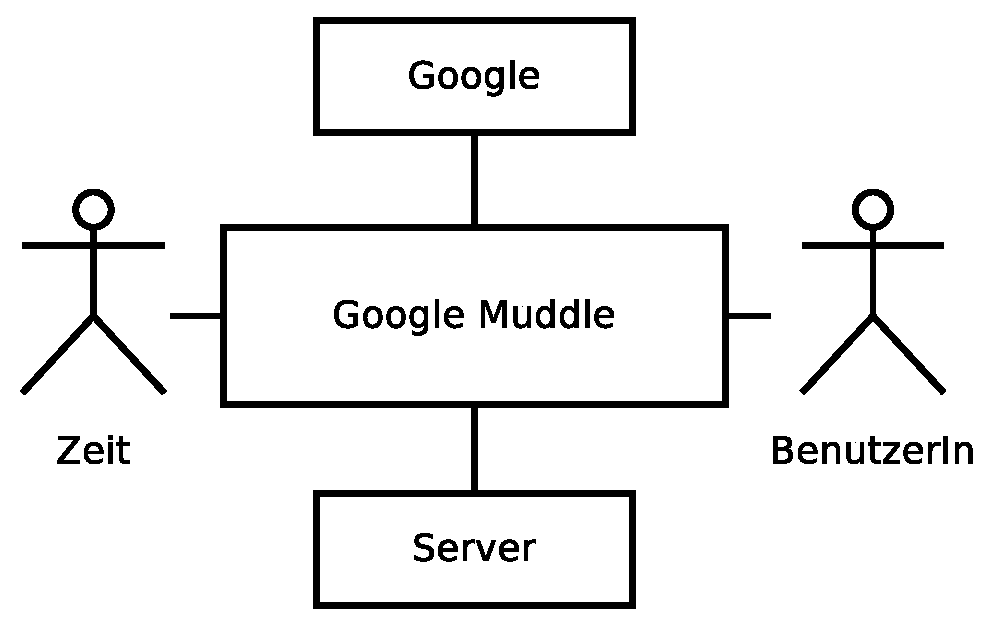
\includegraphics[scale=0.4,clip=]{img/systemkontext.eps}%
\figcaption{Systemkontext \textit{Google Muddle}}%
\label{fig:systemkontext}%
\end{minipage}

\subsection{AkteurInnen}

\subsubsection*{Zeit}

Die Zeit kann zu festgelegten Zeiten oder in bestimmten Intervallen
Anwendungsfälle auslösen.

\subsubsection*{BenutzerIn}

Mit BenutzerIn ist die Person gemeint, welche einen Browser mit \textit{Google
Muddle} als Erweiterung verwendet. Der/die BenutzerIn gilt als AkteurIn,
interagiert aber nur indirekt (über den Browser) mit dem System \textit{Google
Muddle}.

\subsection{Umsysteme}

\subsubsection*{Google}

Anwendungsfälle werden mit der Suchmaschine von Google interagieren.

\subsubsection*{Server}

Die Server-Komponente von \textit{Google Muddle}, welche hier (im Rahmen dieser
Modularbeit) nicht spezifiziert wird, wird ebenfalls mit der Applikation
interagieren.

\newpage
\section{Anwendungsfälle}
\label{sec:anwendungsfaelle}

Das folgende Diagramm (Abbildung \ref{fig:anwendungsfaelle}) gibt eine Übersicht
über alle Anwendungsfälle. Diese werden im Einzelnen in Kapitel
\ref{sec:ablaufbeschreibung} als Ablaufbeschreibungen genauer erläutert.
\\[\intextsep]
\begin{minipage}{\linewidth}
\centering%
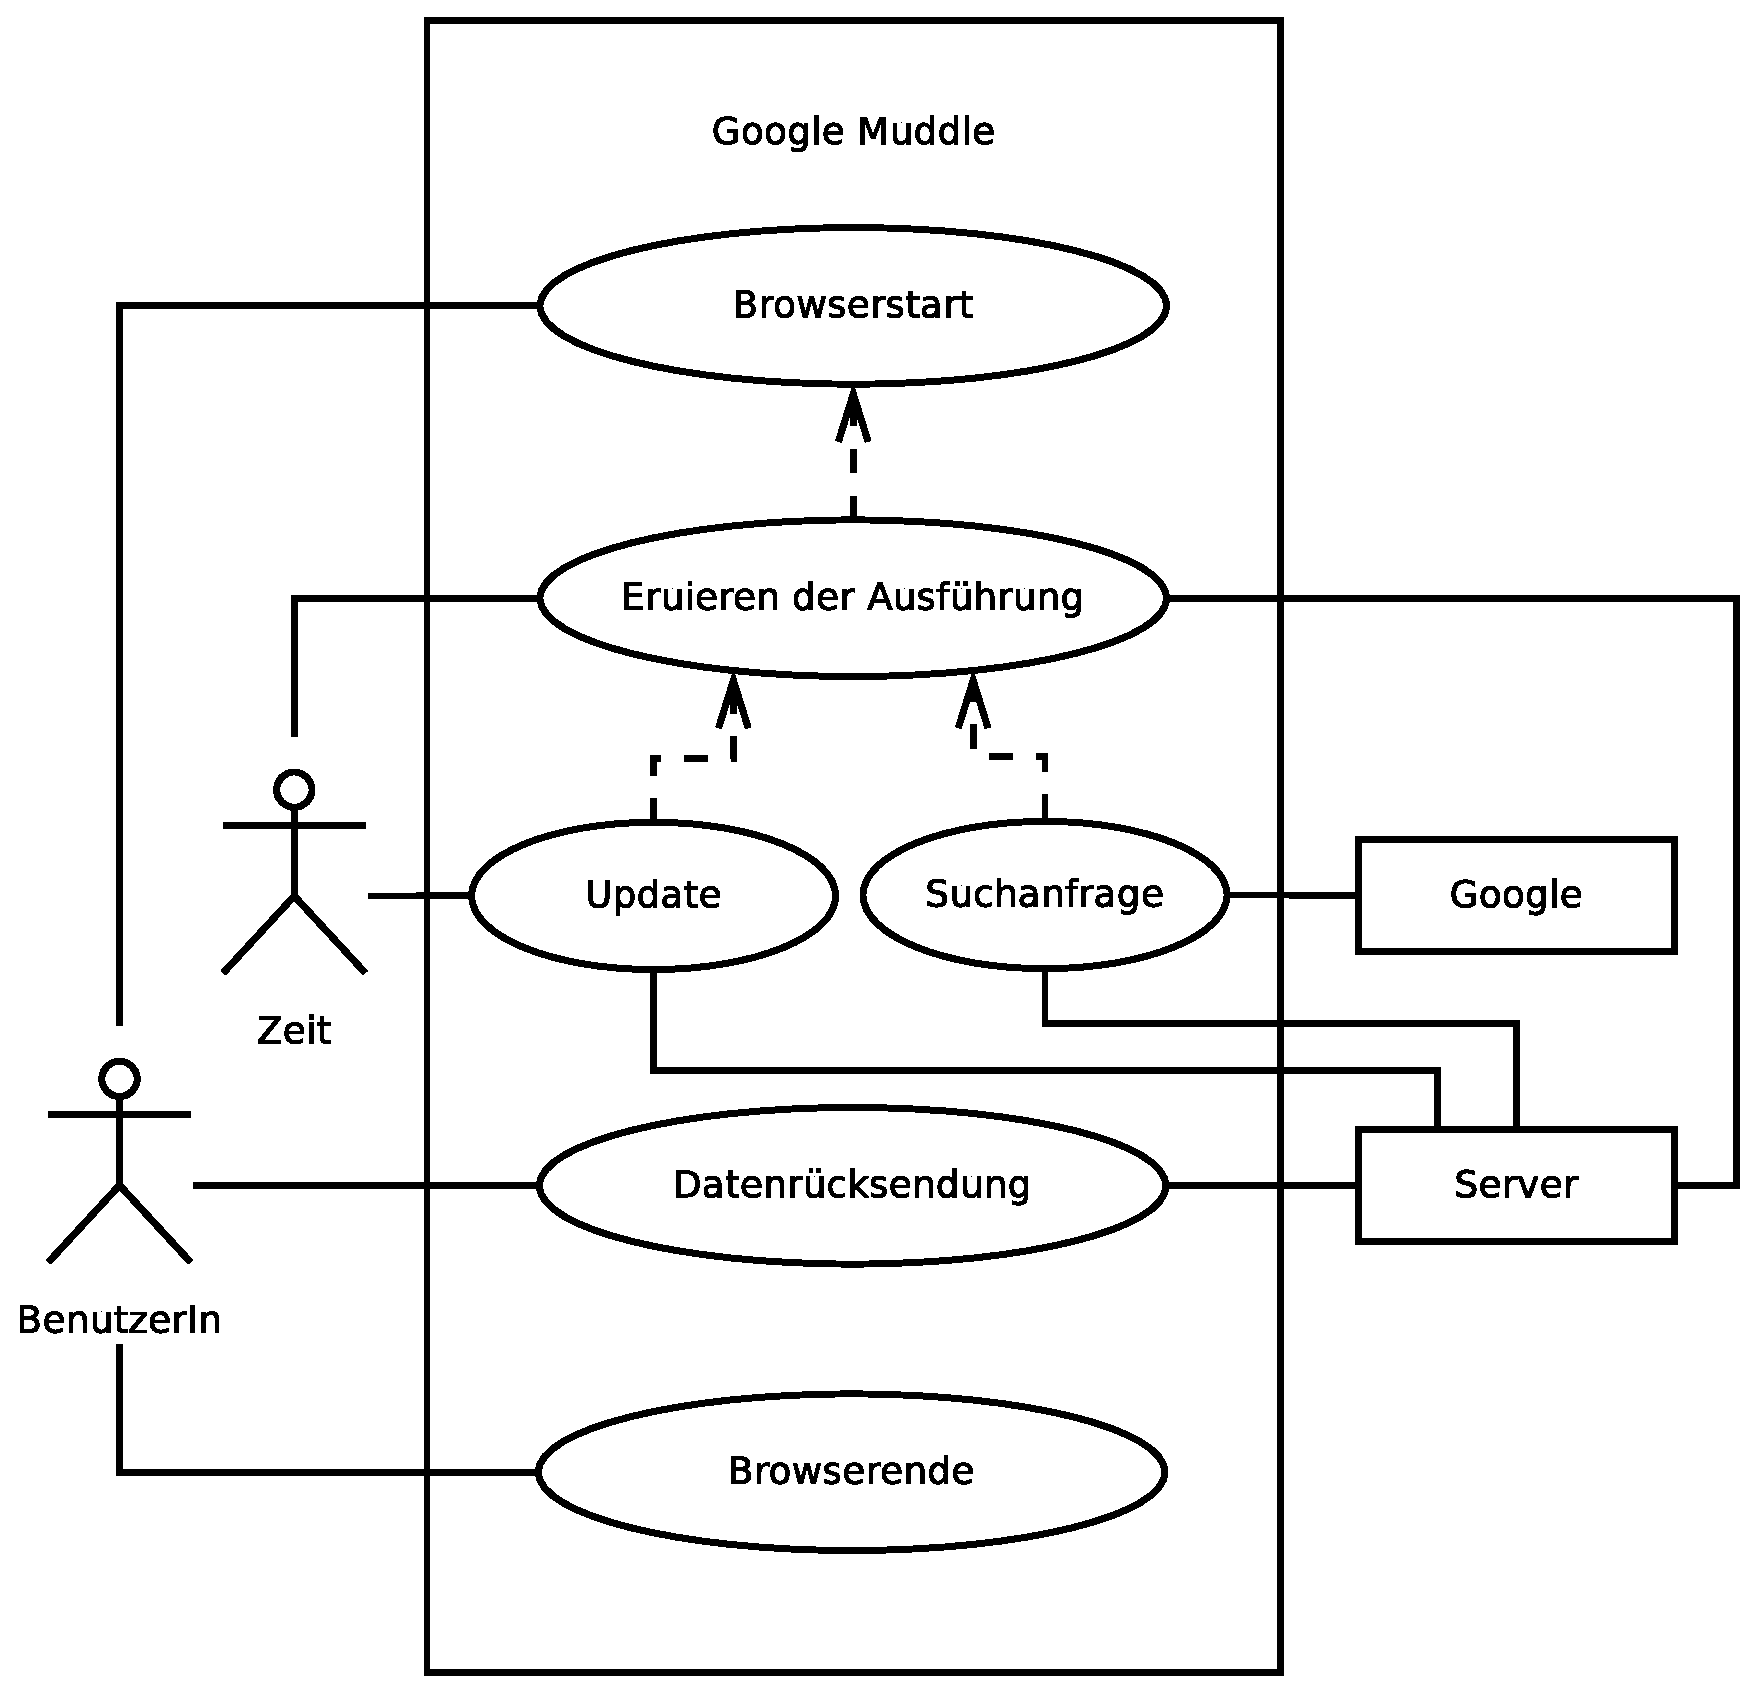
\includegraphics[scale=0.4,clip=]{img/anwendungsfaelle.eps}%
\figcaption{Anwendungsfälle \textit{Google Muddle}}%
\label{fig:anwendungsfaelle}%
\end{minipage}


\newpage
\section{Systemschnittstellen}
\label{sec:systemschnittstellen}

Die Systemschnittstellen werden im Rahmen der Modularbeit nicht erfasst.

\newpage
\section{Ablaufbeschreibung}
\label{sec:ablaufbeschreibung}

Im folgenden sind Ablaufbeschreibungen für die Anwendungsfälle Browserstart,
Eruieren der Ausführung und Suchanfrage zu finden. Die übrigen Anwendungsfälle
werden im Rahmen dieser Modularbeit nicht genauer erfasst. 

Die Diagramme sind als Aktivitätsdiagramme - wie auch alle weiteren Diagramme in
diesem Dokument - nach der \acs{UML} verfasst\footnote[1]{Die \acs{UML} wurde
als geeignete Modellierungssprache ausgewählt, da sie relativ verbreitet ist,
einen einheitlichen Standard für eine grosse Anzahl von Diagrammtypen bietet und
weil viel Literatur dazu gefunden werden kann, was das erarbeiten der Syntax und
Semantik auch für Leute ohne grosse Vorkentnisse stark erleichtert.}.

\subsection{Browserstart}

In Abbildung \ref{fig:ablauf-start} ist der Ablauf für den Anwendungsfall
\enquote{Browserstart} in Bezug auf den für \textit{Google Muddle} relevanten
Teil genauer beschrieben.
\\[\intextsep]
\begin{minipage}{\linewidth}
\centering%
\includegraphics[scale=0.4,clip=]{img/ablauf-start.eps}%
\figcaption{Ablaufbeschreibung Browserstart}%
\label{fig:ablauf-start}%
\end{minipage}

\newpage

\subsection{Eruieren der Ausführung}

Abbildung \ref{fig:ablauf-ausfuehrung} zeigt die Ablaufbeschreibung für den
Anwendungsfall \enquote{Eruieren der Ausführung}.
\\[\intextsep]
\begin{minipage}{\linewidth}
\centering%
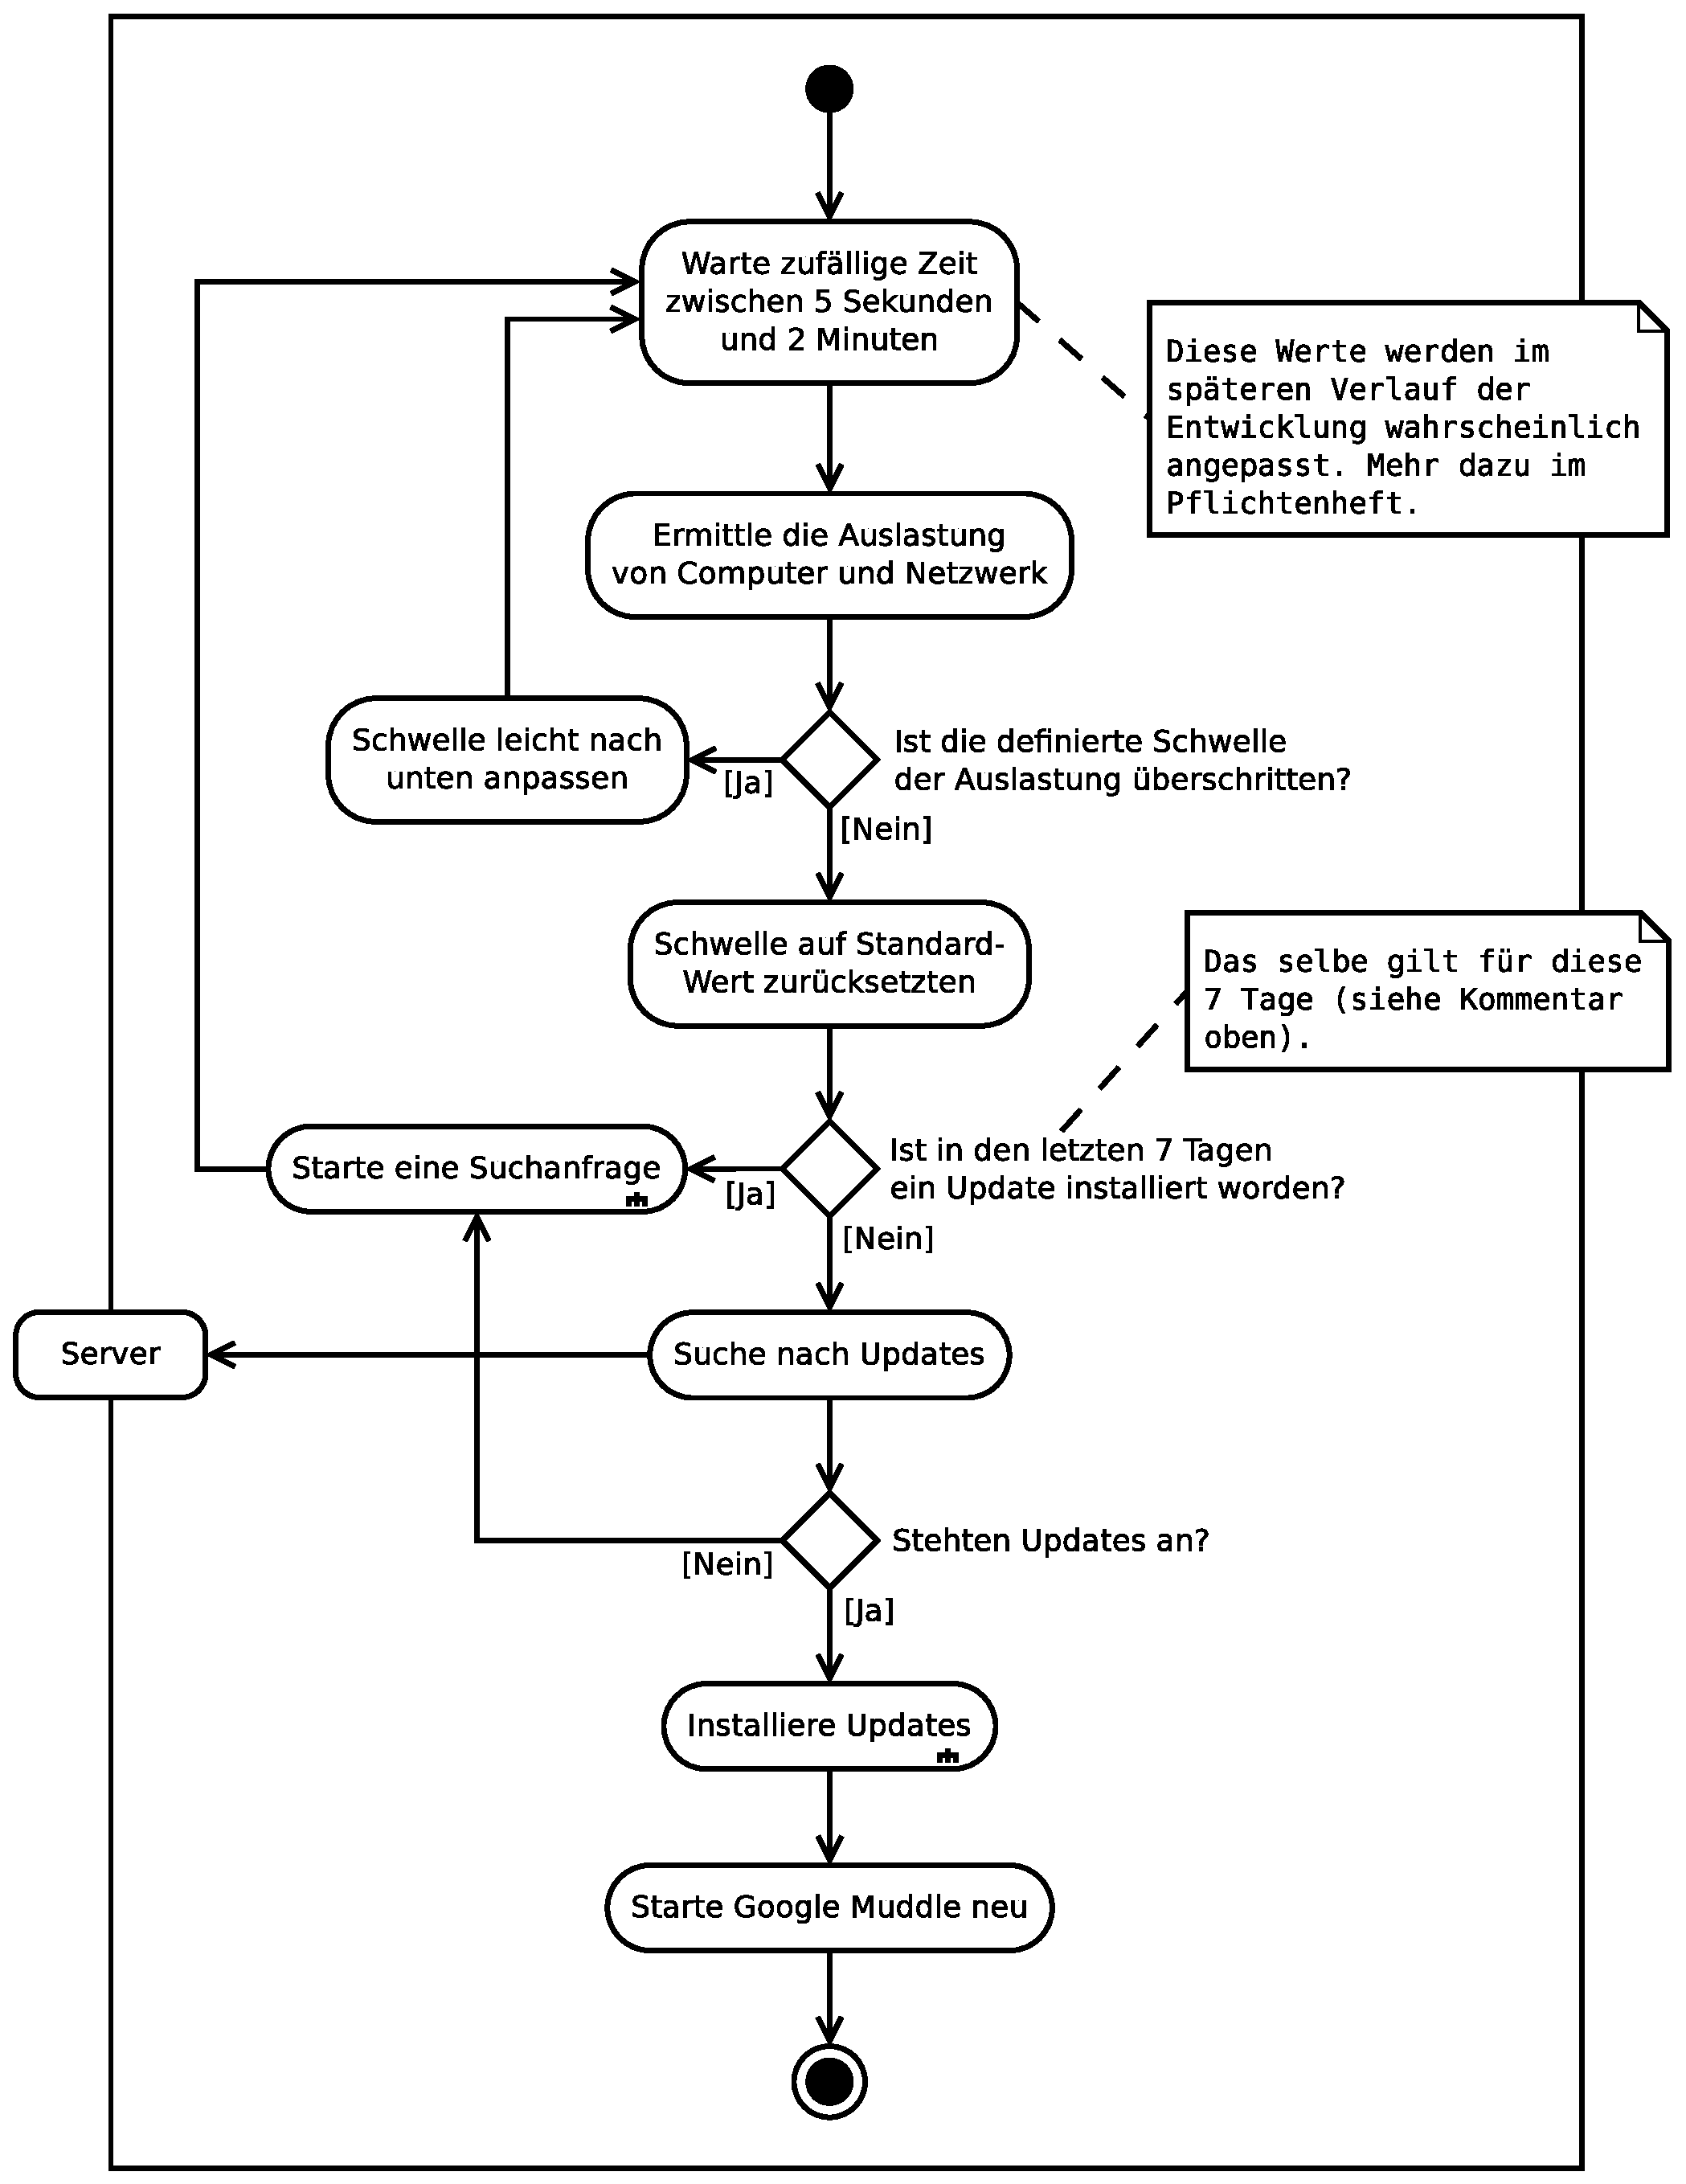
\includegraphics[scale=0.4,clip=]{img/ablauf-ausfuehrung.eps}%
\figcaption{Ablaufbeschreibung Eruieren der Ausführung}%
\label{fig:ablauf-ausfuehrung}%
\end{minipage}

\newpage

\subsection{Suchanfrage}

In Abbildung \ref{fig:ablauf-suche} wird die Ablaufbeschreibung für den
Anwendungsfall \enquote{Suchanfrage} dargestellt.
\\[\intextsep]
\begin{minipage}{\linewidth}
\centering%
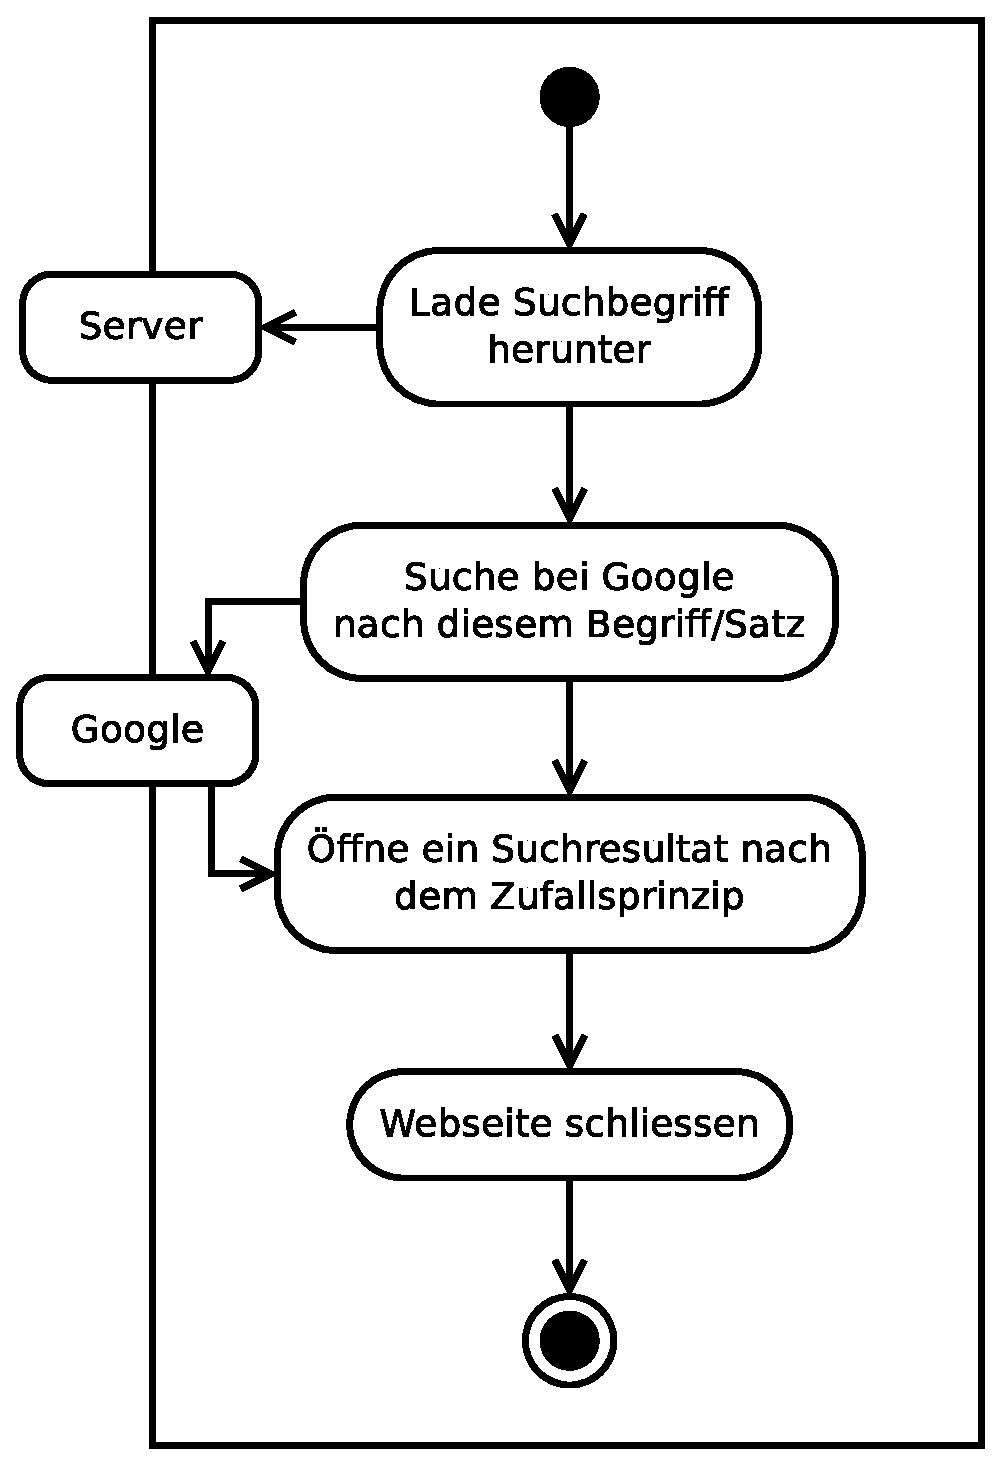
\includegraphics[scale=0.4,clip=]{img/ablauf-suche.eps}%
\figcaption{Ablaufbeschreibung Suchanfrage}%
\label{fig:ablauf-suche}%
\end{minipage}

\newpage

\subsection{Datenrücksendung}

Diese Ablaufbeschreibung wird im Rahmen der Modularbeit nicht erfasst.

\subsection{Update}

Diese Ablaufbeschreibung wird im Rahmen der Modularbeit nicht erfasst.

\subsection{Browserende}

Diese Ablaufbeschreibung wird im Rahmen der Modularbeit nicht erfasst.


\newpage
\section{Klassendiagramm}
\label{sec:klassendiagramm}

Da die Applikation keinerlei BenutzerInneninteraktion vorsieht und auch kaum
Daten konsistent speichern noch in irgendeiner Form manipulieren muss, fällt das
Klassendiagramm sehr knapp aus.

Die Klasse Konfiguration entählt alle Werte, die von der Applikation konsitent
(z.B. im lokalen Dateisystem) gespeichert werden sollen und die keiner anderen
Klasse logisch zugeordnet werden können.

Die Klasse Suchbegriff ist abstrakt. Sie definiert lediglich ein Attribut,
welches sie an die Klassen Suchwort und Suchsatz vererbt. Der Suchbegriff ist
also entweder ein Suchwort, oder ein Suchsatz. Dies hängt vom Rückgabewert und
somit von der Implementation der Server-Komponente ab, welche in dieser Arbeit
nicht spezifiziert wird.

Das Suchwort sowie der Suchsatz besitzen keine eigenen Attribute. Ihr einziges
Attribut erben sie vom Suchbegriff, nämlich den Text, welcher das Wort bzw.
den Satz für die Suchanfrage bei Google beinhaltet. Getrennt wurden die beiden
Klassen aus logischen Gründen, um bestmögliche Modifizierbarkeit zu
gewährleisten (siehe dazu die nichtfunktionalen Anforderungen im Pflichtenheft).

Die Klasse Suchergebnis steht in folgender Beziehung zum Suchbegriff: Jedes
Suchergebnis hat genau einen Suchbegriff, jeder Suchbegriff hat beliebig viele
Suchergebnisse.
\\[\intextsep]
\begin{minipage}{\linewidth}
\centering%
\includegraphics[scale=0.4,clip=]{img/klassendiagramm.eps}%
\figcaption{Klassendiagramm}%
\label{fig:klassendiagramm}%
\end{minipage}

\newpage

\section*{Abkürzungen}
\begin{acronym}[TDMA]
	\setlength{\itemsep}{-\parsep}
	\acro{UML}{Unified Modelling Language}
	\acro{URL}{Uniform Resource Locator}
\end{acronym}

\listoftables

\listoffigures


\end{document}
